\chapter{Πειράματα - Αποτελέσματα}
\label{chapter:experiments}

Τα πειράματα χωρίζονται στις τρεις φάσεις της υλοποίησης. Οι φάσεις είναι οι εξής:

\begin{itemize}
    \setlength\itemsep{-0.2em}
    \item επιτυχία εντοπισμού κάθε πόρτας του χώρου
    \item επιλογή βέλτιστης σειράς επίσκεψης των δωματίων
    \item πλήρης κάλυψη του χάρτη
\end{itemize}



\section{Πειράματα Εύρεσης Δωματίων}
\label{sec:experiments_map_annotation}

Στο πρώτο μέρος των πειραμάτων χρησιμοποιούνται 80 διαφορετικοί χάρτες με σκοπό την μελέτη της ακρίβειας εύρεσης των διάφορων πορτών του χώρου. Οι 74 συλλέχθηκαν από το \cite{li2019houseexpo}, ενώ για τους υπόλοιπους 6 δημιουργήθηκε το αντίστοιχο περιβάλλον στο Gazebo και μετά από την διαδικασία SLAM προέκυψαν τα αντίστοιχα OGM.

Σε όλους τους χάρτες δοκιμάστηκε η υλοποίηση του προηγουμένου κεφαλαίου \ref{section:map_annotation} και μετρήθηκαν 3 συνολικά στοιχεία:

\begin{itemize}
    \setlength\itemsep{-0.2em}
    \item True Positives: σημεία που είναι πόρτες και εντοπίστηκαν σωστά
    \item False Negatives: σημεία που είναι πόρτες αλλά δεν εντοπίστηκαν
    \item False Positives: σημεία που δεν είναι πόρτες αλλά χαρακτηρίστηκαν ως τέτοιες
\end{itemize}

Στο \autoref{fig:rooms_3_ogm_room_detection_example} παρουσιάζονται από δύο παραδείγματα για κάθε περίπτωση. Έστω ότι στον χάρτη αυτό προέκυψαν 4 τελικοί κόμβοι πόρτας (2 μπλε και 2 κόκκινοι). Οι δύο που σημειώνονται με κόκκινο χρώμα πράγματι βρίσκονται σε πόρτες του δωματίου, δηλαδή είναι True Positives. Οι δύο μπλε κόμβοι δεν αποτελούν σημείο πόρτας αν και έχουν χαρακτηριστεί έτσι, επομένως είναι False Positive. Τέλος, στις περιπτώσεις που σημειώνονται με πράσινους κύκλους η διαδικασία απέτυχε να εντοπίσει τις δύο πόρτες, δηλαδή πρόκειται για περιπτώσεις Fasle Negative αποτελεσμάτων.


\begin{figure}[!htb]
    \centering
    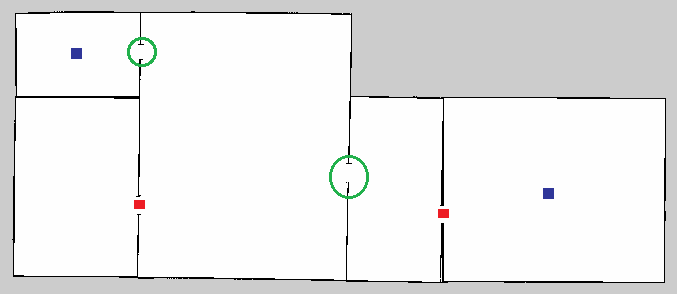
\includegraphics[width=0.8\textwidth]{./images/chapter6/rooms_3_ogm_room_detection_example.png}
    \caption{Παραδείγματα μετρήσεων πειράματος}
    \label{fig:rooms_3_ogm_room_detection_example}
\end{figure}


Τα τελικά αποτελέσματα είναι:
\begin{table}[H]
  \begin{center}
    \caption{Μετρήσεις Εντοπισμού Πορτών}
    \label{tab:room_detection}
    \begin{tabular}{ |>{\columncolor[gray]{0.8}} c | c | }
      \hline
      True Positive & $501$ \\ \hline
      False Negative & $40$ \\ \hline
      False Positive & $149$ \\
      \hline
    \end{tabular}
  \end{center}
\end{table}

Το θετικό συμπέρασμα που προκύπτει είναι ότι η διαδικασία έχει πολύ υψηλό ποσοστό εντοπισμού μιας πόρτας $accuracy = 92.606\%$. Το αρνητικό είναι ότι εμφανίζονται αρκετά συχνά πόρτες σε σημεία που δεν υπάρχουν. Ωστόσο, όπως θα φανεί και από κάποια παραδείγματα δεν είναι τόσο σημαντικό πρόβλημα για δύο λόγους. Πρώτον, πολλές φορές εμφανίζονται παραπάνω πόρτες σε σημέια όπως η μέση ενός διαδρόμου, όπου δεν επηρεάζει αρνητικά την διαδικασία η θεώρηση ενός ακόμη δωματίου. Δεύτερον και σημαντικότερον, η ύπαρξη αυτή προκύπτει εξαιτίας της αναπαράστασης του χώρου. Η συλλογή \cite{li2019houseexpo} περιέχει χάρτες σε μορφή εικόνας png και όχι σε μορφή OGM. Αυτό έχει ως αποτέλεσμα τα σημεία που είναι εκτός των δωματίων, αντί να αντιστοιχούν σε τιμές αγνώστου, αντιστοιχούν σε τιμές εμποδίων. Έτσι, ο αλγόριθμος όταν ελέγχει το ποσοστό κάλυψης της προέκτασης της ευθείας των κοντινότερων εμποδίων δίνει μεγάλες τιμές, κάτι που με κανονική OGM αναπαράσταση δεν θα συνέβαινε. Το επιχείρημα αυτό βασίζεται στο γεγονός ότι και οι έξι OGM χάρτες έχουν 100\% ακρίβεια στον εντοπισμό των πορτών, χωρίς την ύπαρξη λανθασμένων υποδείξεων.

Επομένως, τα δωμάτια ενός χώρου συνδέονται άμεσα με τα χαρακτηριστικά του αντίστοιχου χάρτη. Ο εντοπισμός και διαχωρισμός τους μπορεί να πραγματοποιηθεί με μεγάλη επιτυχία με το αναπτυγμένο σύστημα που εξαρτάται αποκλειστικά από τον εκάστοτε χάρτη.

Στην συνέχεια παρουσιάζονται ορισμένα παραδείγματα χαρτών με τους κόμβους. Οι μπλε κόμβοι αποτελούν τα εκτιμώμενα σημεία πόρτας, τα πράσινα τους υποψήφιους κόμβους πόρτες που απορρίφθηκαν και τα κόκκινα τα υπόλοιπα σημεία του τοπολογικού χάρτη του χώρου.

Στο \ref{fig:room_detection_example_1} επιτεύχθηκε σωστός εντοπισμός των δωματίων. Στο \ref{fig:room_detection_example_2} παρατηρούνται τρεις περιττοί κόμβοι, δύο πάνω αριστερά και ένας κάτω αριστερά. Και οι τρεις προκύπτουν από το γεγονός ότι στο αριστερό μέρος του χώρου υπάρχει ένα τεράστιο εμπόδιο, κάτι που υπό φυσιολογικές συνθήκες θα ήταν άγνωστη περιοχή ή ένα άλλο δωμάτιο. Στο \ref{fig:room_detection_example_3} ο χώρος προσομοιώνει μια πραγματική αποθήκη και η διαδικασία εντοπίζει και τις δύο πόρτες του χώρου. Τέλος, στο \ref{fig:room_detection_example_4} συναντάται ένας πολύ σύνθετος χώρος. Ωστόσο, η διαδικασία εντοπίζει με επιτυχία και τις έξι πόρτες. 

Παρατηρώντας τα παραδείγματα αυτά φαίνεται ότι πράγματι η διαδικασία λειτουργεί με ικανοποιητικά αποτελέσματα σε πολλούς και σύνθετους χώρους όπως είναι μια αποθήκη.


\begin{figure}[!htb]
    \centering
    \begin{subfigure}{0.5\textwidth}
        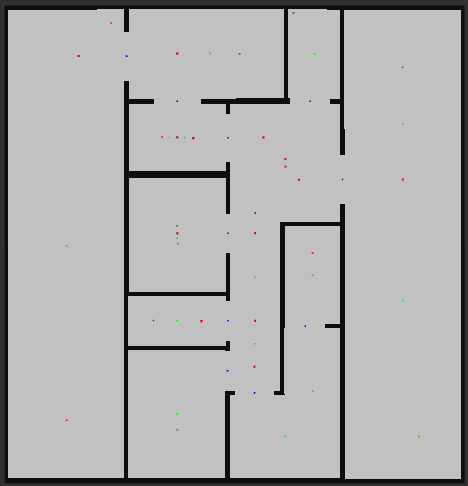
\includegraphics[width=0.9\textwidth]{./images/chapter6/b1c86b70b59c42219161174de6500049.png}
        \caption{Παράδειγμα 1}
        \label{fig:room_detection_example_1}
    \end{subfigure}%
% \end{figure}
% \begin{figure}[!htb]
    \begin{subfigure}{0.5\textwidth}
        \centering
        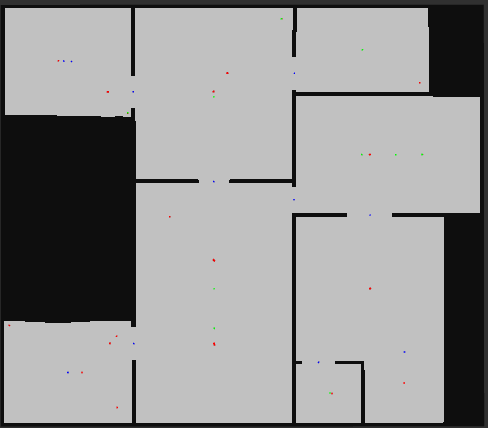
\includegraphics[width=0.9\textwidth]{./images/chapter6/fea87120e90bbffd5e8c42e3b6002165.png}
        \caption{Παράδειγμα 2}
        \label{fig:room_detection_example_2}
    \end{subfigure}
    \begin{subfigure}{0.5\textwidth}
        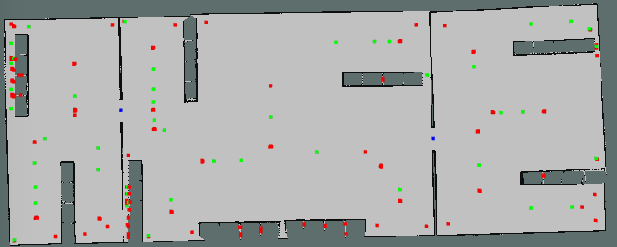
\includegraphics[width=0.9\textwidth]{./images/chapter6/warehouse_2.png}
        \caption{Παράδειγμα 3}
        \label{fig:room_detection_example_3}
    \end{subfigure}%
    \begin{subfigure}{0.5\textwidth}
        \centering
        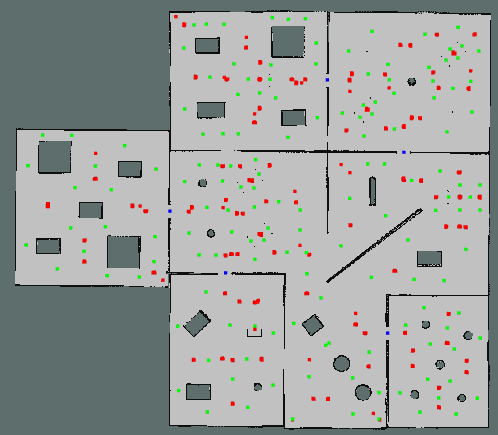
\includegraphics[width=0.9\textwidth]{./images/chapter6/indoor_with_distance_features.png}
        \caption{Παράδειγμα 4}
        \label{fig:room_detection_example_4}
    \end{subfigure}
\end{figure}







\section{Πειράματα Ακολουθίας Δωματίων}
\label{sec:experiments_room_sequence}

Στο δέυτερο μέρος των πειραμάτων χρησιμοποιούνται 70 χάρτες από αυτούς που χρησιμοποιήθηκαν και στο πρώτο μέρος των πειραμάτων με σκοπό τη μελέτη του μήκους της διαδρομής επίσκεψης των δωματίων κάθε χώρου. Συγκρίθηκαν 3 διαφορετικοί αλγόριθμοι, οι:

\begin{itemize}
    \setlength\itemsep{-0.2em}
    \item Επιλογή Κοντινότερου Επόμενου Δωματίου (Κοντινότερος Γείτονας)
    \item Anneal Hill Climb
    \item Random Restart Hill Climb
\end{itemize}

Ο πρώτος αποτελεί μια άπληστη μέθοδο επιλογής, όπου κάθε φορά επιλέγεται ο τρέχων καλύτερος επόμενος κόμβος στην ακολουθία, δηλαδή ο κοντινότερος. Είναι μια απλή και γρήγορη αλλά υποβέλτιστη μέθοδος, εφαρομογή ουσιαστικά του αλγορίθμου επιλογής κοντινότερου γείτονα. Οι δύο άλλοι αναπτύχθηκαν στην \autoref{subsection:room_sequence_implementation} και η σύγκριση τους με την άπληστη μέθοδο καταδεικνύει την αποτελεσματικότητα τους. Επίσης, επισημαίνεται ότι οι δύο HC αλγόριθμοι εκτελέστηκαν για πλήθος επαναλήψεων ίσο με 500 φορές επί το πλήθος των πορτών του χάρτη. Σημαντική παρατήρηση είναι ότι ο χρόνος εκτέλεσης και των τριών αλγορίθμων είναι παρόμοιος και αμελητέος.


Ορισμένα τελικά αποτελέσματα μήκους της συνολικής ακολουθίας επίσκεψης των πορτών σε τιμές brushfire, δηλαδή σε μήκος πάνω στο εκάστοτε OGM είναι:


\begin{longtable}{| p{.20\textwidth} | p{.20\textwidth} | p{.20\textwidth} | p{.20\textwidth} |}

    \caption{Επιλεγμένα Αποτελέσματα Μήκους Ακολουθίας Δωματίων}
    \label{tab:room_sequence_results}
    \hline
    \rowcolor[gray]{0.8}
    Κοντινότερος Γείτονας & Anneal HC & RRHC & Ποσοστό Βελτίωσης με RRHC \\ \hline
    $2809$ & $5201$ & $2809$ & $0$\%\\ \hline
    $3338$ & $6870$ & $2979$ & $10.6$\%\\ \hline
    $7928$ & $11990$ & $7698$ & $2.9$\%\\ \hline
    $2414$ & $2766$ & $2318$ & $3.9$\%\\ \hline
    $2769$ & $4087$ & $2519$ & $9.0$\%\\ \hline
    $2834$ & $3766$ & $2834$ & $0$\%\\ \hline
    $11466$ & $13762$ & $10331$ & $9.8$\%\\ \hline
    $996$ & $996$ & $849$ & $14.7$\%\\ \hline
    $558$ & $558$ & $558$ & $0$\%\\ \hline
    $1149$ & $1149$ & $849$ & $26.1$\%\\ 
    \hline
\end{longtable}



Από τα πειράματα προέκυψαν τα παρακάτω ευρήματα. Αρχικά, ο αλγόριθμος anneal HC τις περισσότερες φορές δίνει αποτέλεσμα σημαντικά μεγαλύτερο από το απλό εξαιτίας της στοχαστικότητας του, κάτι που τελικά τον θέτει μη ικανοποιητικό. Μόλις σε 12 χάρτες, στις πιο απλές περιπτώσεις, οι τιμές του anneal HC ήταν ίσες με τις τιμές του κοντινότερου γείτονα. 

Επιπλέον, ο RRHC δίνει σταθερά ίδια ή καλύτερα αποτελέσματα από τον αλγόριθμο κοντινότερου γείτονα, επομένως, αποτελεί μια σημαντική βελτιωμένη διαδικασία. Σε απλές περιπτώσεις ή περιπτώσεις με μικρό αριθμό δωματίων τα αποτελέσματα των δύο αλγορίθμων είναι συνήθως ίσα, ωστόσο όσο αυξάνεται το πλήθος των δωματίων και μια βέλτιστη λύση γίνεται πιο σύνθετη, τόσο σημαντιότερη είναι η διαφορά των αποτελεσμάτων τον δύο αλγορίθμων. Συγκεκριμένα, σε 31 χάρτες παρατηρήθηκε βελτίωση στο μήκος της διαδρομής, ενώ στους υπόλοιπους 39 τα αποτελέσματα ήταν ίσα. Κατά μέσο όρο το ποσοστό βελτίωσης του μήκους της διαδρομής είναι $7.597$\% στους χάρτες που πράγματι παρουσιάζεται βελτίωση και $3.256$\% συνολικά, ενώ τα τρία μεγαλύτερα ποσοστά είναι $26.1$\%, $15.9$\% και $14.7$\%.



Τα συνολικά αποτελέσματα είναι:
\begin{table}[H]
  \begin{center}
    \caption{Μετρήσεις Μήκους Ακολουθίας Δωματίων}
    \label{tab:room_detection}
    \begin{tabular}{ |>{\columncolor[gray]{0.8}} c | c | }
      \hline
      Χάρτες που παρουσίασαν βελίωση & $31\ /\ 70$ \\ \hline
      Μέση Τιμή βελτίωσης & $3.256\%$ \\ \hline
      Τυπική απόκλιση βελτίωσης & $5.166\%$ \\
      \hline
    \end{tabular}
  \end{center}
\end{table}

Συμπερασματικά, ο anneal HC δεν προσφέρει κάποια βελτίωση, ενώ αντίθετα ο RRHC οδηγεί σε ικανοποιητικά αποτελέσματα και από τη στιγμή που δεν επιφέρει χρονική καθυστέρηση συγκριτικά με απλούστερες μεθόδους, όπως του κοντινότερου γείτονα, μπορεί να χρησιμοποιηθεί για τον υπολογισμό της βέλτιστης ακολουθίας δωματίων κάθε χάρτη.

% %\newpage
\section{Πλήρης Κάλυψη Χώρου}
\label{section:full_coverage}

Η πλήρης κάλυψη ενός χάρτη OGM, αλλά και ενός χώρου γενικότερα, συνεπάγεται την κάλυψη κάθε σημείου του χώρου του χάρτη αυτού. Όπως διατύπωσαν οι Galceran και Carreras \cite{Galceran2013ASO} υπάρχουν έξι προϋποθέσεις για να καλυφθεί βέλτιστα ένας χώρος.
\begin{itemize}
    \setlength\itemsep{-0.2em}
    \item Το ρομπότ πρέπει να περάσει απ' όλα τα σημεία του χώρου, καλύπτοντας τα πλήρως.
    \item Το ρομπότ πρέπει να καλύψει την περιοχή δίχως την ύπαρξη αλληλοεπικαλυπτόμενων περιοχών.
    \item Απαιτούνται συνεχείς και ακολουθιακές διεργασίες, δίχως επαναλήψεις μονοπατιών.
    \item Το ρομπότ πρέπει να αποφεύγει τα εμπόδια του περιβάλλοντος.
    \item Πρέπει να χρησιμοποιούνται όσο το δυνατόν πιο απλές τροχιές κίνησης, όπως ευθείες.
    \item Προτιμάται ένα βέλτιστο μονοπάτι, εαν αυτό υπάρχει.
\end{itemize}

Όμως, το πρόβλημα εύρεσης της βέλτιστης διαδρομής ενός συνόλου σημείων αποτελεί \emph{το πρόβλημα του περιπλανώμενου πωλητή} (Traveling Salesman Problem - TSP) και είναι NP-hard πρόβλημα. Γι' αυτό έχουν αναπτυχθεί απόλυτες μέθοδοι που διαχωρίζουν τον χώρο σε μικρότερα χωρία και επιλύουν βέλτιστα το πρόβλημα της κάλυψης άνα χωρίο, αλλά και ευριστικές μέθοδοι που προσπαθούν να απλοποιήσουν σημαντικά το πρόβλημα και πολλές φορές δεν φτάνουν σε μια βέλτιστη λύση.

Μια από τις πρώτες προσεγγίσεις που δημοσιεύτηκαν είναι των Choset και Pignon \cite{Choset1998}. Αυτοί πρότειναν την μέθοδο της αποσύνθεσης του χώρου με την κινήση boustrophedon, την κίνηση δηλαδή που κάνει ένα βόδι σε ένα χωράφι. Οι περιοχές οι οποίες περιλαμβάνουν εμπόδια δεν επιτρέπουν την ύπαρξη μιας συνεχόμενης διαδρομής. Γι' αυτό, ο χώρος χωρίζεται σε επιμέρους τμήματα και στο εσωτερικό τους πραγματοποιείται η συγκεκριμένη κίνηση. Έτσι, καλύπτονται τα σημεία του χώρου με απλές κινήσεις του ρομποτικού οχήματος προς τα μπροστά και προς τα πίσω. Μόλις καλυφθεί κάθε σημείο, αυτομάτως έχει καλυφθεί ολόκληρος ο χώρος.

Στο \cite{brown2016} χρησιμοποιείται μια παραλλαγή της boustrophedon μεθόδου. Εδώ σε κάθε χώρο σχηματίζεται μια σπειροειδής διαδρομή που ξεκινάει από το κέντρο του δωματίου και τερματίζει στην πόρτα του. Μετά συνδιάζονται όλες οι διαδρομές των δωματίων, ώστε το συνολικό μονοπάτι να είναι βέλτιστο.

Όπως αναφέρεται στο \cite{Galceran2013ASO}, υπάρχουν και άλλες τεχνικές διαχωρισμού του χώρου εκτός του boustrophedon. Υπάρχει ο διαχωρισμός Morse, ο τραπεζοειδής διαχωρισμός, ο διαχωρισμός Morse κάνοντας χρήση και του GVD κ.α.

Οι ευριστικές μέθοδοι χρησιμοποιούν διάφορα μοτίβα για να καλύψουν πλήρως τον χώρο. Oι Faud και Purwanto \cite{fuad2014} χρησιμοποιώντας την εικόνα της κάμερας του ρομπότ το κατευθύνουν να ακουλουθεί τους τοίχους των διαδρόμων (wall following) διατηρώντας από αυτούς μια σταθερή απόσταση. Έτσι, πραγματοποιεί έμμεσα την πλήρη κάλυψη αυτών των χώρων.



